% -----------------------------*- LaTeX -*------------------------------
\documentclass[UTF8]{report}
% ------------------------------------------------------------------------
% Packages
% ------------------------------------------------------------------------
\usepackage{ctex} % 支持中文
\usepackage[body={7in, 9in},left=1in,right=1in]{geometry} % 改变页边距
\usepackage{amsmath} % AMS 的数学宏包
\usepackage{amsfonts} % AMS 的数学字体宏包
\usepackage{amssymb} % AMS 符号库
\usepackage{bm} % 数学公式中的黑斜体
\usepackage{amsthm} % AMS 的定理环境宏包
\usepackage{graphicx} % 插图
\usepackage{subfigure} % 插子图
\usepackage{nicefrac} % 好看的分数
\usepackage{mathrsfs} % mathscr font
\usepackage{caption} % caption
\usepackage{algorithm,algorithmicx} % 伪代码支持宏包
\usepackage[noend]{algpseudocode} % 伪代码
\usepackage{fancyhdr} % 设置页眉、页脚
\usepackage{adjustbox} % 图片尺寸自动调整
\usepackage{esint} % 积分符号
\usepackage{mathtools} % 数学宏包的重要补充
\usepackage{upgreek} % 数学环境的直立希腊字母
\usepackage{enumitem} % 使用enumitem宏包, 改变列表项的格式
\usepackage{color} % 支持彩色
\usepackage{extarrows} % 任意长度的箭头
\usepackage{tikz} % 绘图
\usepackage{forest} % 绘树
\usepackage{xcolor} % 颜色宏包
\usepackage{breqn} % 公式自动换行
\usepackage{fontsize} % 字体大小
\usepackage[framemethod=TikZ]{mdframed} % 给文字加框
\usepackage{fontspec} % 字体库
\usepackage{bigstrut} % 用于表格中的换行
\usepackage{multirow} % 表格中多行单元格合并
\usepackage{multicol} % 表格中多列单元格合并
\usepackage{longtable} % 长表格
\usepackage{rotating} % 旋转图形和表格      以上三者用于绘制三线表
\usepackage{booktabs} % 三线表宏包
\usepackage{scribe} % Scribe 模板
\usepackage{diagbox} % 表格斜线
\usepackage{listings} % 插入代码
\usepackage{verbatim} % 多行注释
\usepackage{ifplatform} % 检测编译平台
\usetikzlibrary{shapes.geometric, arrows} % 引入流程图需要的库
\usetikzlibrary{automata} % 引入automata库
\usetikzlibrary{shapes,arrows,positioning,chains} % 引入positioning库
% ------------------------------------------------------------------------
% Macros
% ------------------------------------------------------------------------
%~~~~~~~~~~~~~~~
% Utility latin
%~~~~~~~~~~~~~~~
\newcommand{\ie}{\textit{i.e.}}
\newcommand{\eg}{\textit{e.g.}}
%~~~~~~~~~~~~~~~
% Environment shortcuts
%~~~~~~~~~~~~~~~
\newcommand{\balign}[1]{\ealign{\begin{align}#1\end{align}}}
\newcommand{\baligns}[1]{\ealigns{\begin{align*}#1\end{align*}}}
\newcommand{\bitemize}[1]{\eitemize{\begin{itemize}#1\end{itemize}}}
\newcommand{\benumerate}[1]{\eenumerate{\begin{enumerate}#1\end{enumerate}}}
%~~~~~~~~~~~~~~~
% Text with quads around it
%~~~~~~~~~~~~~~~
\newcommand{\qtext}[1]{\quad\text{#1}\quad}
%~~~~~~~~~~~~~~~
% Shorthand for math formatting
%~~~~~~~~~~~~~~~
\newcommand{\mbb}[1]{\mathbb{#1}}
\newcommand{\mbi}[1]{\boldsymbol{#1}} % Bold and italic (math bold italic)
\newcommand{\mbf}[1]{\mathbf{#1}}
\newcommand{\mc}[1]{\mathcal{#1}}
\newcommand{\mrm}[1]{\mathrm{#1}}
\newcommand{\tbf}[1]{\textbf{#1}}
\newcommand{\tsc}[1]{\textsc{#1}}
%\def\\langle {{\langle }}
%\def\\rangle {{\rangle }}
\newcommand{\sT}{\sf T}
\newcommand{\grad}{\nabla}
\newcommand{\Proj}{\Pi}
%~~~~~~~~~~~~~~~
% Common sets 定义数集符号
%~~~~~~~~~~~~~~~
\newcommand{\R}{\mathbb{R}}
\newcommand{\Z}{\mathbb{Z}}
\newcommand{\Q}{\mathbb{Q}}
\newcommand{\N}{\mathbb{N}}
\newcommand{\C}{\mathbb{C}}
\newcommand{\reals}{\mathbb{R}} % Real number symbol
\newcommand{\integers}{\mathbb{Z}} % Integer symbol
\newcommand{\rationals}{\mathbb{Q}} % Rational numbers
\newcommand{\naturals}{\mathbb{N}} % Natural numbers
\newcommand{\complex}{\mathbb{C}} % Complex numbers
%~~~~~~~~~~~~~~~
% Common functions
%~~~~~~~~~~~~~~~
\renewcommand{\exp}[1]{\operatorname{exp}\left(#1\right)} % Exponential
\newcommand{\indic}[1]{\mbb{I}\left(#1\right)} % Indicator function
\newcommand{\indicsub}[2]{\mbb{I}_{#2}\left(#1\right)} % Indicator function
\newcommand{\argmax}{\mathop\mathrm{arg\, max}} % Defining math symbols
\newcommand{\argmin}{\mathop\mathrm{arg\, min}}
\renewcommand{\arccos}{\mathop\mathrm{arccos}}
\newcommand{\dom}{\mathop\mathrm{dom}} % Domain
\newcommand{\range}{\mathop\mathrm{range}} % Range
\newcommand{\diag}{\mathop\mathrm{diag}}
\newcommand{\tr}{\mathop\mathrm{tr}}
\newcommand{\abs}{\mathop\mathrm{abs}}
\newcommand{\card}{\mathop\mathrm{card}}
\newcommand{\sign}{\mathop\mathrm{sign}}
\newcommand{\prox}{\mathrm{prox}} % prox
\newcommand{\rank}[1]{\mathrm{rank}(#1)}
\newcommand{\supp}[1]{\mathrm{supp}(#1)}
\newcommand{\norm}[1]{\lVert#1\rVert}
%~~~~~~~~~~~~~~~
% Common probability symbols
%~~~~~~~~~~~~~~~
\newcommand{\family}{\mathcal{P}} % probability family / statistical model
\newcommand{\iid}{\stackrel{\mathrm{iid}}{\sim}}
\newcommand{\ind}{\stackrel{\mathrm{ind}}{\sim}}
\newcommand{\E}{\mathbb{E}} % Expectation symbol
\newcommand{\Earg}[1]{\E\left[#1\right]}
\newcommand{\Esubarg}[2]{\E_{#1}\left[#2\right]}
\renewcommand{\P}{\mathbb{P}} % Probability symbol
\newcommand{\Parg}[1]{\P\left(#1\right)}
\newcommand{\Psubarg}[2]{\P_{#1}\left[#2\right]}
%\newcommand{\Cov}{\mrm{Cov}} % Covariance symbol
%\newcommand{\Covarg}[1]{\Cov\left[#1\right]}
%\newcommand{\Covsubarg}[2]{\Cov_{#1}\left[#2\right]}
%\newcommand{\model}{\mathcal{P}} % probability family / statistical model
%~~~~~~~~~~~~~~~
% Distributions
%~~~~~~~~~~~~~~~
%\newcommand{\Gsn}{\mathcal{N}}
%\newcommand{\Ber}{\textnormal{Ber}}
%\newcommand{\Bin}{\textnormal{Bin}}
%\newcommand{\Unif}{\textnormal{Unif}}
%\newcommand{\Mult}{\textnormal{Mult}}
%\newcommand{\NegMult}{\textnormal{NegMult}}
%\newcommand{\Dir}{\textnormal{Dir}}
%\newcommand{\Bet}{\textnormal{Beta}}
%\newcommand{\Gam}{\textnormal{Gamma}}
%\newcommand{\Poi}{\textnormal{Poi}}
%\newcommand{\HypGeo}{\textnormal{HypGeo}}
%\newcommand{\GEM}{\textnormal{GEM}}
%\newcommand{\BP}{\textnormal{BP}}
%\newcommand{\DP}{\textnormal{DP}}
%\newcommand{\BeP}{\textnormal{BeP}}
%\newcommand{\Exp}{\textnormal{Exp}}
%~~~~~~~~~~~~~~~
% Theorem-like environments
%~~~~~~~~~~~~~~~
%\theoremstyle{definition}
%\newtheorem{definition}{Definition}
%\newtheorem{example}{Example}
%\newtheorem{problem}{Problem}
%\newtheorem{lemma}{Lemma}
%~~~~~~~~~~~~~~~
% 组合数学的模板和作业里用到的一些宏包和自定义命令
%~~~~~~~~~~~~~~~
\renewcommand{\emph}[1]{\begin{kaishu}#1\end{kaishu}}
\newcommand{\falfac}[1]{^{\underline{#1}}}
\newcommand{\binomfrac}[2]{\frac{#1^{\underline{#2}}}{#2!}}
\newcommand{\ceil}[1]{\left\lceil #1 \right\rceil}
\newcommand{\floor}[1]{\left\lfloor #1 \right\rfloor}
\newcommand{\suminfty}[2]{\sum_{#1=#2}^{\infty}}
\newcommand{\suminftyk}[0]{\sum_{k=0}^{\infty}}
\newcommand{\sumint}[3]{\sum_{#1=#2}^{#3}}
\newcommand{\sumintk}[2]{\sum_{k=#1}^{#2}}
\newcommand{\suminti}[2]{\sum_{i=#1}^{#2}}
%~~~~~~~~~~~~~~~
% 定义新命令
%~~~~~~~~~~~~~~~
\newcommand*{\unit}[1]{\mathop{}\!\mathrm{#1}}
\newcommand*{\dif}{\mathop{}\!\mathrm{d}}%微分算子 d
\newcommand*{\pdif}{\mathop{}\!\partial}%偏微分算子
\newcommand*{\cdif}{\mathop{}\!\nabla}%协变导数、nabla 算子
\newcommand*{\laplace}{\mathop{}\!\Delta}%laplace 算子
\newcommand*{\deri}[1]{\mathrm{d} #1}
\newcommand*{\deriv}[2]{\frac{\mathrm{d} #1}{\mathrm{d} {#2}}}
\newcommand*{\derivh}[3]{\frac{\mathrm{d}^{#1} #2}{\mathrm{d} {#3^{#1}}}}
\newcommand*{\pderiv}[2]{\frac{\partial #1}{\partial {#2}}}
\newcommand*{\pderivh}[3]{\frac{\partial^{#1} #2}{\partial {#3^{#1}}}}
\newcommand*{\dderiv}[2]{\dfrac{\mathrm{d} #1}{\mathrm{d} {#2}}}
\newcommand*{\dderivh}[3]{\dfrac{\mathrm{d}^{#1} #2}{\mathrm{d} {#3^{#1}}}}
\newcommand*{\dpderiv}[2]{\dfrac{\partial #1}{\partial {#2}}}
\newcommand*{\dpderivh}[3]{\dfrac{\partial^{#1} #2}{\partial {#3^{#1}}}}
\newcommand{\me}[1]{\mathrm{e}^{#1}}%e 指数
\newcommand{\mi}{\mathrm{i}}%虚数单位
%\newcommand{\mc}{\mathrm{c}}%光速 定义与mathcal冲突
\newcommand{\red}[1]{\textcolor{red}{#1}}
\newcommand{\blue}[1]{\textcolor{blue}{#1}}
%\newcommand{\Rome}[1]{\setcounter{rome}{#1}\Roman{rome}}
%~~~~~~~~~~~~~~~
% 公式环境中箭头符号的简写
%~~~~~~~~~~~~~~~
\newcommand{\ra}{\rightarrow}
\newcommand{\Ra}{\Rightarrow}
\newcommand{\la}{\leftarrow}
\newcommand{\La}{\Leftarrow}
\newcommand{\lra}{\leftrightarrow}
\newcommand{\Lra}{\Leftrightarrow}
\newcommand{\lgla}{\longleftarrow}
\newcommand{\Lgla}{\Longleftarrow}
\newcommand{\lgra}{\longrightarrow}
\newcommand{\Lgra}{\Longrightarrow}
\newcommand{\lglra}{\longleftrightarrow}
\newcommand{\Lglra}{\Longleftrightarrow}
%~~~~~~~~~~~~~~~
% 一些数学的环境设置
%~~~~~~~~~~~~~~~
%\newcounter{counter_exm}\setcounter{counter_exm}{1}
%\newcounter{counter_prb}\setcounter{counter_prb}{1}
%\newcounter{counter_thm}\setcounter{counter_thm}{1}
%\newcounter{counter_lma}\setcounter{counter_lma}{1}
%\newcounter{counter_dft}\setcounter{counter_dft}{1}
%\newcounter{counter_clm}\setcounter{counter_clm}{1}
%\newcounter{counter_cly}\setcounter{counter_cly}{1}
\newtheorem{theorem}{{\hskip 1.7em \bf 定理}}
\newtheorem{lemma}[theorem]{\hskip 1.7em 引理}
\newtheorem{proposition}[theorem]{\hskip 1.7em 命题}
\newtheorem{claim}[theorem]{\hskip 1.7em 断言}
\newtheorem{corollary}[theorem]{\hskip 1.7em 推论}
% \newcommand{\problem}[1]{{\setlength{\parskip}{10pt}\noindent \bf{#1}}}
\newenvironment{solution}{{\noindent \bf 解 \quad}}{}
\newenvironment{remark}{{\noindent \bf 注 \quad}}{}
\newenvironment{definition}{{\noindent \bf 定义 \quad}}{}
\renewenvironment{proof}{{\setlength{\parskip}{7pt}\noindent\hskip 2em \bf 证明 \quad}}{\hfill$\qed$\par}
\newenvironment{example}{{\noindent\bf 例 \quad}}{\hfill$\qed$\par}
%\newenvironment{concept}[1]{{\bf #1\quad} \begin{kaishu}} {\end{kaishu}\par}
%~~~~~~~~~~~~~~~
% 本.tex文档中特殊定义命令
%~~~~~~~~~~~~~~~
\newcommand{\lno}[1]{\overline{#1}}
\newcommand{\NP}{\mathrm{NP}}
\newcommand{\coNP}{\mathrm{coNP}}
% \newcommand{\ISO}{\mathrm{ISO}}
\newcommand{\SAT}{\mathrm{SAT}}
\newcommand{\USAT}{\mathrm{USAT}}
% \newcommand{\threeSAT}{\mathrm{3\text{-}SAT}}
\renewcommand{\P}{\mathrm{P}}
% \mathchardef\mhyphen="2D
% \newcommand{\CNF}{\mathrm{CNF}}
% \newcommand{\DNF}{\mathrm{DNF}}
% \newcommand{\SetSp}{\mathrm{SET\text{-}SPLITTING}}
% \newcommand{\PUZZLE}{\mathrm{PUZZLE}}
% \newcommand{\SPATH}{\mathrm{SPATH}}
% \newcommand{\LPATH}{\mathrm{LPATH}}
% \newcommand{\UHAMPATH}{\mathrm{UHAMPATH}}
\newcommand{\SPACE}{\mathrm{SPACE}}
\newcommand{\NSPACE}{\mathrm{NSPACE}}
\newcommand{\PSPACE}{\mathrm{PSPACE}}
\newcommand{\NPSPACE}{\mathrm{NPSPACE}}
\newcommand{\DFA}{\mathrm{DFA}}
\newcommand{\NFA}{\mathrm{NFA}}
\newcommand{\TQBF}{\mathrm{TQBF}}
% \newcommand{\L}{\mathrm{L}}
\renewcommand{\O}{\mathrm{O}}
\newcommand{\NL}{\mathrm{NL}}
\newcommand{\coNL}{\mathrm{coNL}}
\newcommand{\LADDER}{\mathrm{LADDER_{DFA}}}
\newcommand{\hd}{\mathrm{\text{-}hard}}
\newcommand{\ADD}{\mathrm{ADD}}
\newcommand{\STCN}{\mathrm{STRONGLY\text{-}CONNECTED}}
\newcommand{\PATH}{\mathrm{PATH}}
\newcommand{\A}{\mathrm{A}}
%使用align环境公式换页
\allowdisplaybreaks[4]

\definecolor{dkgreen}{rgb}{0,0.6,0}
\definecolor{gray}{rgb}{0.5,0.5,0.5}
\definecolor{mauve}{rgb}{0.58,0,0.82}
\lstset{
  frame=tb,
  aboveskip=3mm,
  belowskip=3mm,
  showstringspaces=false,
  columns=flexible,
  framerule=1pt,
  rulecolor=\color{gray!35},
  backgroundcolor=\color{gray!5},
  basicstyle={\small\ttfamily},
  numbers=left,
  numberstyle=\ttfamily\color{gray},
  keywordstyle=\color{blue},
  commentstyle=\color{dkgreen},
  stringstyle=\color{mauve},
  breaklines=true,
  breakatwhitespace=true,
  tabsize=3,
}

\lstdefinelanguage{LoongArch}{
  morekeywords={la, lw, addi, sw, li, syscall, beqz, add, move, bge, blt, b, sub, ret, beq, bne},  
  literate={ll.w}{{{\color{blue}ll.w}}}1
           {sc.w}{{{\color{blue}sc.w}}}1
           {addi.d}{{{\color{blue}addi.d}}}1
           {st.d}{{{\color{blue}st.d}}}1
           {st.w}{{{\color{blue}st.w}}}1
           {ldptr.w}{{{\color{blue}ldptr.w}}}1
           {slli.d}{{{\color{blue}slli.d}}}1
           {ld.d}{{{\color{blue}ld.d}}}1
           {stptr.w}{{{\color{blue}stptr.w}}}1
           {slli.w}{{{\color{blue}slli.w}}}1
           {ld.w}{{{\color{blue}ld.w}}}1
           {addi.w}{{{\color{blue}addi.w}}}1
           {add.d}{{{\color{blue}add.d}}}1
           {sub.w}{{{\color{blue}sub.w}}}1
           {li.w}{{{\color{blue}li.w}}}1
           {bstrpick.d}{{{\color{blue}bstrpick.d}}}1
           {alsl.d}{{{\color{blue}alsl.d}}}1,
  morecomment=[l]{\#},
  frame=tb,
  aboveskip=3mm,
  belowskip=3mm,
  showstringspaces=false,
  columns=flexible,
  framerule=1pt,
  rulecolor=\color{gray!35},
  backgroundcolor=\color{gray!5},
  basicstyle={\small\ttfamily},
  numbers=left,
  numberstyle=\ttfamily\color{gray},
  keywordstyle=\color{blue},
  commentstyle=\color{dkgreen},
  stringstyle=\color{mauve},
  breaklines=true,
  breakatwhitespace=true,
  tabsize=3,
}

\tikzstyle{startstop} = [rectangle, rounded corners, minimum width=3cm, minimum height=1cm,text centered, draw=black, fill=red!30]
\tikzstyle{process} = [rectangle, minimum width=3cm, minimum height=1cm, text centered, draw=black, fill=orange!30]
\tikzstyle{decision} = [diamond, minimum width=3cm, minimum height=1cm, text centered, draw=black, fill=green!30]
\tikzstyle{arrow} = [thick,->,>=stealth]

\ifwindows
    \setmainfont{Times New Roman}
    \setsansfont{Times New Roman}
    \setmonofont{Consolas}
    \setCJKmainfont{SimHei}
    \setCJKsansfont{SimSun}
    \setCJKmonofont{FangSong}
\fi

\ifmacosx
    \setmainfont{Times New Roman}
    \setsansfont{Times New Roman}
    \setmonofont{Menlo}
    \setCJKmainfont{STHeiti}
    \setCJKsansfont{STSong}
    \setCJKmonofont{STFangsong}
\fi

\punctstyle{kaiming}

\begin{document}

\pagestyle{fancy}

\reporttype{Homework}                 % required
\course{Computer Architecture} 				% optional
\coursetitle{Hardware-Software Codesign}	    % optional
\semester{Fall 2024}			    % optional
\lecturer{Hu Weiwu}			% optional
\scribe{Zhang Jiawei}			% required
\lecturenumber{4}				% required (must be a number)
\lecturedate{September 30}			% required (omit year)
\maketitle


\noindent
\textbf{4.1}

在Linux/LoongArch64 ABI 的函数调用约定中,\texttt{(char)0x61}以整型调用,参数使用寄存器\$a0-\$a7传递;\texttt{(short)0xfff}以整型调用,参数使用寄存器\$a0-\$a7传递;\texttt{1}以整型调用,参数使用寄存器\$a0-\$a7传递;\texttt{2}以整型调用,参数使用寄存器\$a0-\$a7传递;\texttt{3.0}以浮点型调用,参数使用寄存器\$fa0-\$fa7传递;\texttt{4.0}以浮点型调用,参数使用寄存器\$fa0-\$fa7传递;\texttt{sm}以整型调用,参数使用寄存器\$a0-\$a7传递;\texttt{bg}超过2XLEN位,以整型调用,参数使用引用传递;\texttt{9}以整型调用,参数使用寄存器\$a0-\$a7传递。

\noindent
\textbf{4.2}

\begin{enumerate}[label=(\arabic*)]
  \item 举例如下:
  
  \begin{lstlisting}[language=LoongArch]
    # 线程1和线程2均运行以下代码
    _start: 
      la      $t0, counter       # 加载 counter 的地址到 t0
      lw      $t1, 0($t0)         # 从 counter 加载当前值到 t1
      addi    $t1, $t1, 1         # t1 = t1 + 1
      sw      $t1, 0($t0)         # 将 t1 的值存回 counter
  \end{lstlisting}

  显然,两个线程可能同时读取\texttt{counter}的值,然后同时对其进行加一操作,导致最终的结果不正确。

  \item 使用LL/SC指令改写程序片段:
  
  \begin{lstlisting}[language=LoongArch]
    # 线程1和线程2均运行以下代码
    _start:
      la      $t0, counter       # 加载 counter 的地址到 t0
    atomic_add:  
      ll.w    $t1, 0($t0)         # 加载链接:从 counter 加载当前值到 t1
      addi    $t2, $t1, 1         # t2 = t1 + 1
      sc.w    $t2, $t2, 0(t0)     # 存储条件:尝试将 t2 存回 counter
      beqz    t2, atomic_add    # 如果存储失败,重试
  \end{lstlisting}

  使用LL/SC指令实现自旋锁,可以保证对\texttt{counter}的操作是原子的,从而避免了多线程并发问题。
\end{enumerate}

\noindent
\textbf{4.3}

安装LoongArch交叉编译器后,先使用\texttt{loongarch64-unknown-linux-gnu-gcc}编译C程序,再使用\texttt{loongarch64-unknown-linux-gnu-objdump -d}查看反汇编代码。我所写C程序如下:
  
  \begin{lstlisting}[language=C]
    #include <stdio.h>

    int bubble_sort(int *arr, int n) {
        int i, j, temp;
        for (i = 0; i < n - 1; i++) {
            for (j = 0; j < n - i - 1; j++) {
                if (arr[j] > arr[j + 1]) {
                    temp = arr[j];
                    arr[j] = arr[j + 1];
                    arr[j + 1] = temp;
                }
            }
        }
        return 0;
    }
    
    int main() {
        int arr[] = {64, 34, 25, 12, 22, 11, 90};
        int n = sizeof(arr) / sizeof(arr[0]);
        bubble_sort(arr, n);
        printf("Sorted array: \n");
        for (int i = 0; i < n; i++) {
            printf("%d ", arr[i]);
        }
        printf("\n");
        return 0;
    }
  \end{lstlisting}

  使用-O0优化(不优化)反汇编代码中冒泡排序函数部分如下:

  \begin{lstlisting}[language=LoongArch]
    000000000000083c <bubble_sort>:
    83c:	02ff4063 	addi.d      	$sp, $sp, -48
    840:	29c0a076 	st.d        	$fp, $sp, 40
    844:	02c0c076 	addi.d      	$fp, $sp, 48
    848:	29ff62c4 	st.d        	$a0, $fp, -40
    84c:	001500ac 	move        	$t0, $a1
    850:	29bf52cc 	st.w        	$t0, $fp, -44
    854:	29bfb2c0 	st.w        	$zero, $fp, -20
    858:	5000dc00 	b           	220	# 934 <bubble_sort+0xf8>
    85c:	29bfa2c0 	st.w        	$zero, $fp, -24
    860:	5000a400 	b           	164	# 904 <bubble_sort+0xc8>
    864:	24ffeacc 	ldptr.w     	$t0, $fp, -24
    868:	0041098c 	slli.d      	$t0, $t0, 0x2
    86c:	28ff62cd 	ld.d        	$t1, $fp, -40
    870:	0010b1ac 	add.d       	$t0, $t1, $t0
    874:	2400018e 	ldptr.w     	$t2, $t0, 0
    878:	24ffeacc 	ldptr.w     	$t0, $fp, -24
    87c:	02c0058c 	addi.d      	$t0, $t0, 1
    880:	0041098c 	slli.d      	$t0, $t0, 0x2
    884:	28ff62cd 	ld.d        	$t1, $fp, -40
    888:	0010b1ac 	add.d       	$t0, $t1, $t0
    88c:	2400018c 	ldptr.w     	$t0, $t0, 0
    890:	001501cd 	move        	$t1, $t2
    894:	6400658d 	bge         	$t0, $t1, 100	# 8f8 <bubble_sort+0xbc>
    898:	24ffeacc 	ldptr.w     	$t0, $fp, -24
    89c:	0041098c 	slli.d      	$t0, $t0, 0x2
    8a0:	28ff62cd 	ld.d        	$t1, $fp, -40
    8a4:	0010b1ac 	add.d       	$t0, $t1, $t0
    8a8:	2400018c 	ldptr.w     	$t0, $t0, 0
    8ac:	29bf92cc 	st.w        	$t0, $fp, -28
    8b0:	24ffeacc 	ldptr.w     	$t0, $fp, -24
    8b4:	02c0058c 	addi.d      	$t0, $t0, 1
    8b8:	0041098c 	slli.d      	$t0, $t0, 0x2
    8bc:	28ff62cd 	ld.d        	$t1, $fp, -40
    8c0:	0010b1ad 	add.d       	$t1, $t1, $t0
    8c4:	24ffeacc 	ldptr.w     	$t0, $fp, -24
    8c8:	0041098c 	slli.d      	$t0, $t0, 0x2
    8cc:	28ff62ce 	ld.d        	$t2, $fp, -40
    8d0:	0010b1cc 	add.d       	$t0, $t2, $t0
    8d4:	240001ad 	ldptr.w     	$t1, $t1, 0
    8d8:	2500018d 	stptr.w     	$t1, $t0, 0
    8dc:	24ffeacc 	ldptr.w     	$t0, $fp, -24
    8e0:	02c0058c 	addi.d      	$t0, $t0, 1
    8e4:	0041098c 	slli.d      	$t0, $t0, 0x2
    8e8:	28ff62cd 	ld.d        	$t1, $fp, -40
    8ec:	0010b1ac 	add.d       	$t0, $t1, $t0
    8f0:	28bf92cd 	ld.w        	$t1, $fp, -28
    8f4:	2500018d 	stptr.w     	$t1, $t0, 0
    8f8:	28bfa2cc 	ld.w        	$t0, $fp, -24
    8fc:	0280058c 	addi.w      	$t0, $t0, 1
    900:	29bfa2cc 	st.w        	$t0, $fp, -24
    904:	28bf52cd 	ld.w        	$t1, $fp, -44
    908:	28bfb2cc 	ld.w        	$t0, $fp, -20
    90c:	001131ac 	sub.w       	$t0, $t1, $t0
    910:	0040818c 	slli.w      	$t0, $t0, 0x0
    914:	02bffd8c 	addi.w      	$t0, $t0, -1
    918:	0040818d 	slli.w      	$t1, $t0, 0x0
    91c:	28bfa2cc 	ld.w        	$t0, $fp, -24
    920:	0040818c 	slli.w      	$t0, $t0, 0x0
    924:	63ff418d 	blt         	$t0, $t1, -192	# 864 <bubble_sort+0x28>
    928:	28bfb2cc 	ld.w        	$t0, $fp, -20
    92c:	0280058c 	addi.w      	$t0, $t0, 1
    930:	29bfb2cc 	st.w        	$t0, $fp, -20
    934:	28bf52cc 	ld.w        	$t0, $fp, -44
    938:	02bffd8c 	addi.w      	$t0, $t0, -1
    93c:	0040818d 	slli.w      	$t1, $t0, 0x0
    940:	28bfb2cc 	ld.w        	$t0, $fp, -20
    944:	0040818c 	slli.w      	$t0, $t0, 0x0
    948:	63ff158d 	blt         	$t0, $t1, -236	# 85c <bubble_sort+0x20>
    94c:	0015000c 	move        	$t0, $zero
    950:	00150184 	move        	$a0, $t0
    954:	28c0a076 	ld.d        	$fp, $sp, 40
    958:	02c0c063 	addi.d      	$sp, $sp, 48
    95c:	4c000020 	ret         
  \end{lstlisting}
  
  使用-O1优化反汇编代码中冒泡排序函数部分如下:

  \begin{lstlisting}[language=LoongArch]
    000000000000083c <bubble_sort>:
    83c:	0280040c 	li.w        	$t0, 1
    840:	64006585 	bge         	$t0, $a1, 100	# 8a4 <bubble_sort+0x68>
    844:	004080b0 	slli.w      	$t4, $a1, 0x0
    848:	02800411 	li.w        	$t5, 1
    84c:	02c01092 	addi.d      	$t6, $a0, 4
    850:	50002c00 	b           	44	# 87c <bubble_sort+0x40>
    854:	02c0118c 	addi.d      	$t0, $t0, 4
    858:	58001d8f 	beq         	$t0, $t3, 28	# 874 <bubble_sort+0x38>
    85c:	2400018d 	ldptr.w     	$t1, $t0, 0
    860:	2400058e 	ldptr.w     	$t2, $t0, 4
    864:	67fff1cd 	bge         	$t2, $t1, -16	# 854 <bubble_sort+0x18>
    868:	2500018e 	stptr.w     	$t2, $t0, 0
    86c:	2980118d 	st.w        	$t1, $t0, 4
    870:	53ffe7ff 	b           	-28	# 854 <bubble_sort+0x18>
    874:	02bffe10 	addi.w      	$t4, $t4, -1
    878:	58002e11 	beq         	$t4, $t5, 44	# 8a4 <bubble_sort+0x68>
    87c:	0040820c 	slli.w      	$t0, $t4, 0x0
    880:	64001e2c 	bge         	$t5, $t0, 28	# 89c <bubble_sort+0x60>
    884:	0015008c 	move        	$t0, $a0
    888:	02bffa0f 	addi.w      	$t3, $t4, -2
    88c:	00df01ef 	bstrpick.d  	$t3, $t3, 0x1f, 0x0
    890:	002c81ef 	alsl.d      	$t3, $t3, $zero, 0x2
    894:	0010c9ef 	add.d       	$t3, $t3, $t6
    898:	53ffc7ff 	b           	-60	# 85c <bubble_sort+0x20>
    89c:	02bffe10 	addi.w      	$t4, $t4, -1
    8a0:	53ffdfff 	b           	-36	# 87c <bubble_sort+0x40>
    8a4:	00150004 	move        	$a0, $zero
    8a8:	4c000020 	ret         
  \end{lstlisting}

  使用-O2优化反汇编代码中冒泡排序函数部分如下:

  \begin{lstlisting}[language=LoongArch]
    00000000000008dc <bubble_sort>:
    8dc:	0280040c 	li.w        	$t0, 1
    8e0:	64004d85 	bge         	$t0, $a1, 76	# 92c <bubble_sort+0x50>
    8e4:	004080b0 	slli.w      	$t4, $a1, 0x0
    8e8:	02c01092 	addi.d      	$t6, $a0, 4
    8ec:	02800411 	li.w        	$t5, 1
    8f0:	64004630 	bge         	$t5, $t4, 68	# 934 <bubble_sort+0x58>
    8f4:	02bffa0f 	addi.w      	$t3, $t4, -2
    8f8:	00df01ef 	bstrpick.d  	$t3, $t3, 0x1f, 0x0
    8fc:	002c81ef 	alsl.d      	$t3, $t3, $zero, 0x2
    900:	0015008c 	move        	$t0, $a0
    904:	0010c9ef 	add.d       	$t3, $t3, $t6
    908:	2400018d 	ldptr.w     	$t1, $t0, 0
    90c:	2400058e 	ldptr.w     	$t2, $t0, 4
    910:	64000dcd 	bge         	$t2, $t1, 12	# 91c <bubble_sort+0x40>
    914:	2500018e 	stptr.w     	$t2, $t0, 0
    918:	2980118d 	st.w        	$t1, $t0, 4
    91c:	02c0118c 	addi.d      	$t0, $t0, 4
    920:	5fffe98f 	bne         	$t0, $t3, -24	# 908 <bubble_sort+0x2c>
    924:	02bffe10 	addi.w      	$t4, $t4, -1
    928:	5fffca11 	bne         	$t4, $t5, -56	# 8f0 <bubble_sort+0x14>
    92c:	00150004 	move        	$a0, $zero
    930:	4c000020 	ret         
    934:	02bffe10 	addi.w      	$t4, $t4, -1
    938:	53ffbbff 	b           	-72	# 8f0 <bubble_sort+0x14>
  \end{lstlisting}
  
  使用-O3优化反汇编代码中冒泡排序函数部分与-O2优化反汇编代码相同,故不再重复给出。

  不同的优化级别对编译生成的汇编代码有显著影响:

  -O0:无优化,代码较长,执行效率低,适用于调试。

  -O1:基本优化,代码长度减少,执行效率提升,适用于需要一定优化但仍需调试的场景。

  -O2:较高优化,代码显著减少,执行效率显著提升,适用于大多数应用程序。

  -O3:最高级别优化,进一步优化代码长度和执行效率,适用于对性能要求极高的应用程序。(本题无效果)
  
\noindent
\textbf{4.4}

所写C程序如下:

\begin{lstlisting}[language=C]
  #include <stdio.h>
  struct exp{
      char a;
      short b;
      int c;
      long d;
      float e;
      double f;
      long double g;
  };
  
  int main(){
      struct exp s;
      printf("Size of struct: %lu\n", sizeof(s));
      printf("Size of char: %lu\n", sizeof(s.a));
      printf("Size of short: %lu\n", sizeof(s.b));
      printf("Size of int: %lu\n", sizeof(s.c));
      printf("Size of long: %lu\n", sizeof(s.d));
      printf("Size of float: %lu\n", sizeof(s.e));
      printf("Size of double: %lu\n", sizeof(s.f));
      printf("Size of long double: %lu\n", sizeof(s.g));
      return 0;
  }
\end{lstlisting}

输出结果如下:

\begin{lstlisting}[language=bash]
  Size of struct: 48
  Size of char: 1
  Size of short: 2
  Size of int: 4
  Size of long: 8
  Size of float: 4
  Size of double: 8
  Size of long double: 16
\end{lstlisting}

显然有$48 > 1 + 2 + 4 + 8 + 4 + 8 + 16$,这是由于结构体内部的成员在内存中是按照对齐方式排列的,char类型的成员a占用1字节,short类型的成员b占用2字节,从第2字节开始,int类型的成员c占用4字节,从第4字节开始,long类型的成员d占用8字节,从第8字节开始,float类型的成员e占用4字节,从第12字节开始,double类型的成员f占用8字节,从第16字节开始,long double类型的成员g占用16字节,从第32字节开始,所以结构体的大小为48字节。

更改结构体中的成员顺序:

\begin{lstlisting}[language=C]
  struct exp
  {
      char a;
      long double g;
      short b;
      int c;
      long d;
      float e;
      double f;
  };
\end{lstlisting}

输出结果如下:

\begin{lstlisting}[language=bash]
  Size of struct: 64
  Size of char: 1
  Size of short: 2
  Size of int: 4
  Size of long: 8
  Size of float: 4
  Size of double: 8
  Size of long double: 16
\end{lstlisting}

显然有$64 > 1 + 2 + 4 + 8 + 4 + 8 + 16$,这也是由于结构体内部的成员在内存中是按照对齐方式排列的,char类型的成员a占用1字节,long double类型的成员g占用16字节,从第16字节开始,short类型的成员b占用2字节,从第32字节开始,int类型的成员c占用4字节,从第36字节开始,long类型的成员d占用8字节,从第40字节开始,float类型的成员e占用4字节,从第48字节开始,double类型的成员f占用8字节,从第56字节开始,所以结构体的大小为64字节。

\noindent
\textbf{4.5}

我使用x86汇编,所写程序如下:

\begin{lstlisting}[language={[x86masm]Assembler}]
  section .bss
  buffer resb 1  ; 用于存储输入的字符
  
  section .text
  global _start
  
  _start:
      ; 系统调用号 (sys_read)
      mov rax, 0          ; 系统调用号 (sys_read)
      mov rdi, 0          ; 文件描述符 (stdin)
      mov rsi, buffer     ; 缓冲区地址
      mov rdx, 1          ; 读取的字节数
      syscall             ; 调用内核
  
      ; 系统调用号 (sys_write)
      mov rax, 1          ; 系统调用号 (sys_write)
      mov rdi, 1          ; 文件描述符 (stdout)
      mov rsi, buffer     ; 缓冲区地址
      mov rdx, 1          ; 写入的字节数
      syscall             ; 调用内核
  
      ; 系统调用号 (sys_exit)
      mov rax, 60         ; 系统调用号 (sys_exit)
      xor rdi, rdi        ; 退出状态码
      syscall             ; 调用内核
\end{lstlisting}

通过gdb调试,观察\texttt{sys_read}系统调用前后的寄存器状态:

\begin{figure}[H]
  \centering
  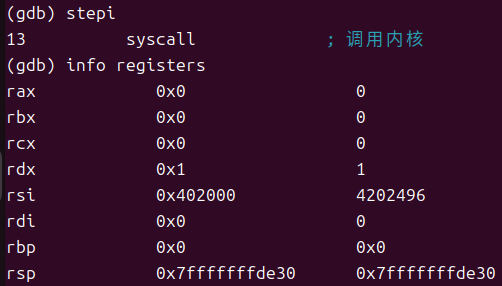
\includegraphics[width=0.6\textwidth]{beforesysread_reg.png}
  \caption{sys\_read系统调用前寄存器状态}
\end{figure}

\begin{figure}[H]
  \centering
  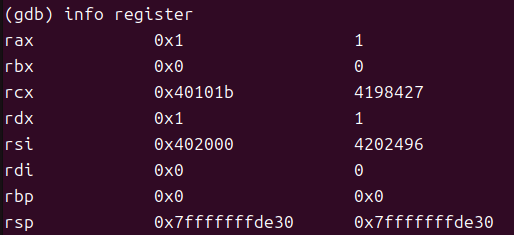
\includegraphics[width=0.6\textwidth]{aftersysread_reg.png}
  \caption{sys\_read系统调用后寄存器状态}
\end{figure}

对照x86的ABI,系统调用号存储在\texttt{rax}寄存器中,文件描述符存储在\texttt{rdi}寄存器中,缓冲区地址存储在\texttt{rsi}寄存器中,读取的字节数存储在\texttt{rdx}寄存器中,且使用syscall指令来触发系统调用。观察gdb调试结果,发现\texttt{rcx}寄存器的值从0变为0x40101b,这是因为\texttt{rcx}寄存器在\texttt{sys_read}系统调用之后被修改为当前指令的pc值,以回到用户态继续执行。
\end{document}